\usetikzlibrary{calc,arrows.meta}
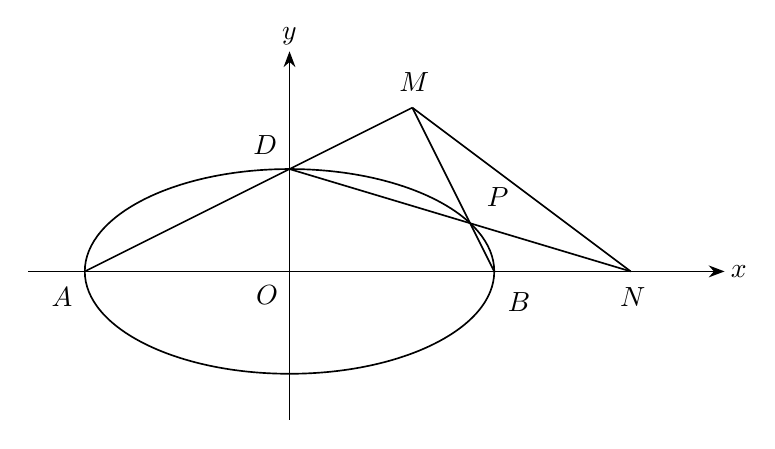
\begin{tikzpicture}[x=1.3cm,y=1.3cm,line width=.6pt,>=Stealth,font=\normalsize]
\coordinate (O) at (0,0);
\coordinate (A) at (-2,0);
\coordinate (B) at (2,0);
\coordinate (D) at (0,1);
\coordinate (P) at (1.7647,0.4706);
\coordinate (M) at (1.2,1.6);
\coordinate (N) at (3.3333,0);
\draw[->] (-2.55,0)--(4.25,0) node[anchor=west,inner sep=0pt,xshift=2pt] {$x$};
\draw[->] (0,-1.45)--(0,2.15) node[anchor=south,inner sep=0pt,yshift=2pt] {$y$};
\draw (O) ellipse [x radius=2, y radius=1];
\draw (A)--(M);
\draw (B)--(M);
\draw (D)--(N);
\draw (M)--(N);
\node[anchor=north east,inner sep=2pt] at ($(O)+(-0.05,-0.08)$) {$O$};
\node[anchor=north east,inner sep=2pt] at ($(A)+(-0.06,-0.10)$) {$A$};
\node[anchor=north west,inner sep=2pt] at ($(B)+(0.07,-0.14)$) {$B$};
\node[anchor=south east,inner sep=2pt] at ($(D)+(-0.06,0.08)$) {$D$};
\node[anchor=south west,inner sep=2pt] at ($(P)+(0.10,0.10)$) {$P$};
\node[anchor=south,inner sep=2pt] at ($(M)+(0.02,0.10)$) {$M$};
\node[anchor=north,inner sep=2pt] at ($(N)+(0.02,-0.10)$) {$N$};
\end{tikzpicture}
